\chapter{CONTEXTUALIZAÇÃO DA INSTITUIÇÃO}
\label{chap:contex}

Este capítulo trata de dados históricos da Universidade Tecnológica Federal do Paraná (UTFPR), o contexto da instituição no estado do Paraná e a instauração do curso de Engenharia Eletrônica no campus da cidade de Toledo.

\section{HISTÓRICO DA UNIVERSIDADE TECNOLÓGICA FEDERAL DO PARANÁ}
\label{sec:hist}

A história da UTFPR teve início no século passado. Sua trajetória começou com a criação das Escolas de Aprendizes Artífices em várias capitais do país, pelo então presidente Nilo Peçanha, em 23 de setembro de 1909. No Paraná, a escola foi inaugurada no dia 16 de janeiro de 1910, em um prédio da Praça Carlos Gomes em Curitiba. O ensino era destinado a garotos de camadas menos favorecidas da sociedade, chamados de ``desprovidos da sorte''. Pela manhã, esses meninos recebiam conhecimentos elementares (primário) e, de tarde, aprendiam ofícios nas áreas de alfaiataria, sapataria, marcenaria e serralheria. Inicialmente, havia 45 estudantes matriculados na escola, que, logo em seguida, instalou seções de Pintura Decorativa e Escultura Ornamental. Aos poucos, a escola cresceu e o número de estudantes aumentou, fazendo com que se procurasse uma sede maior. Então, em 1936, a Instituição foi transferida para a Avenida Sete de Setembro com a Rua Desembargador Westphalen, onde permanece até hoje.

O ensino tornou-se cada vez mais profissional até que, no ano seguinte (1937), a escola começou a ministrar o ensino de 1º grau, sendo denominada Liceu Industrial do Paraná. Cinco anos depois (1942), a organização do ensino industrial foi realizada em todo o país. A partir disso, o ensino passou a ser ministrado em dois ciclos. No primeiro, havia o ensino industrial básico, o de mestria e o artesanal. No segundo, o técnico e o pedagógico. Com a reforma, foi instituída a rede federal de instituições de ensino industrial e o Liceu passou a chamar-se Escola Técnica de Curitiba. Em 1943, tiveram início os primeiros cursos técnicos: Construção de Máquinas e Motores, Edificações, Desenho Técnico e Decoração de Interiores. Antes dividido em ramos diferentes, em 1959, o ensino técnico no Brasil foi unificado pela legislação em vigor.

A escola ganhou, assim, maior autonomia e passou a chamar-se Escola Técnica Federal do Paraná. Em 1974, foram implantados os primeiros cursos de curta duração de Engenharia de Operação (Construção Civil e Elétrica). Quatro anos depois (1978), a Instituição foi transformada em Centro Federal de Educação Tecnológica do Paraná (CEFET-PR), passando a ministrar cursos de graduação plena. A partir da implantação dos cursos superiores, deu-se início ao processo de “maioridade” da Instituição, que avançaria, nas décadas de 80 e 90, com a criação dos Programas de Pós-Graduação. Em 1990, o Programa de Expansão e Melhoria do Ensino Técnico fez com que o CEFET-PR se expandisse para o interior do Paraná, onde implantou unidades. Com a Lei de Diretrizes e Bases da Educação (LDBE) \cite{Lei:9394:1996}, que não permitia mais a oferta dos cursos técnicos integrados, a Instituição, tradicional na oferta desses cursos, decidiu implantar o Ensino Médio e cursos de Tecnologia. Em 1998, em virtude das legislações complementares à LDBE, a diretoria do então CEFET-PR tomou uma decisão ainda mais ousada: criou um projeto de transformação da Instituição em Universidade Tecnológica.

\nomenclature[A]{CEFET-PR}{Centro Federal de Educação Tecnológica do Paraná}
\nomenclature[A]{LDBE}{Lei de Diretrizes e Bases da Educação}

Após sete anos de preparo e o aval do governo federal, o projeto tornou-se lei no dia 7 de outubro de 2005. O CEFET-PR, então, passou a ser a Universidade Tecnológica Federal do Paraná (UTFPR) \cite{Lei:11.184:2005} – a primeira especializada do Brasil. Atualmente, a Universidade Tecnológica conta com 13 campi, distribuídos nas cidades de Apucarana, Campo Mourão, Cornélio Procópio, Curitiba, Dois Vizinhos, Francisco Beltrão, Guarapuava, Londrina,  Medianeira, Pato Branco, Ponta Grossa, Santa Helena e Toledo, conforme mostra a \autoref{fig:13campi}. O \autoref{qua:denomi} apresenta, de forma resumida, as diferentes denominações que a instituição teve ao longo do tempo.

\nomenclature[A]{UTFPR}{Universidade Tecnológica Federal do Paraná}

    \begin{figure}[!htb]
        \centering
        \caption[Localização dos 13 campi da UTFPR]{Localização dos 13 campi da UTFPR no estado do Paraná}
        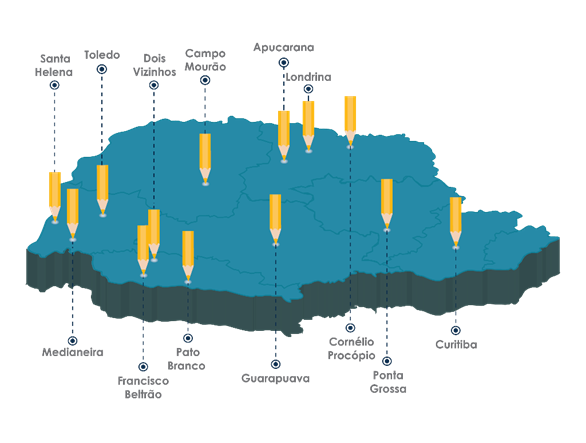
\includegraphics[width=0.7\textwidth]{Caps/Figs/campus_utfpr.png}
        \fonte{\utf}
        \label{fig:13campi}
    \end{figure}
    
    \begin{quadro}[h]
        \centering
        \caption[Diferentes denominações da UTFPR]{As diferentes denominações da UTFPR ao longo de sua existência}        
        \label{qua:denomi}
		\begin{tabularx}{0.7\textwidth}{c >{\centering\arraybackslash}X}
			\toprule%
			\rowcolor{white}\bfseries Ano & \bfseries Denominação\\
			\midrule
			\csvreader[	head to column names,
						late after line=\csvifoddrow{\\}{\\\rowcolor{gray!10}}, 
						separator=pipe]%
						{Caps/Quadros/denominacoesUtfpr.csv}{}%
						{\ano & \denominacao}%
			\bottomrule
			\end{tabularx}
    \end{quadro}

\section{HISTÓRICO DO CAMPUS}

O município de Toledo está situado na região Oeste do Paraná à 555 km de Curitiba e à 1445 km de Brasília. Pela sua localização geográfica, constitui uma área geopolítica estratégica e de relevância para a integração dos povos do Cone Sul da América. A cidade de Toledo possui aproximadamente 144 mil habitantes, conforme estimativa do Instituto Brasileiro de Geografia e Estatística (IBGE) \cite{ibge2020}.

\nomenclature[A]{IBGE}{Instituto Brasileiro de Geografia e Estatistica}

O município de Toledo é polo microrregional, sede da 18\textordfeminine{} Região Administrativa do Estado do Paraná, congregando 21 municípios que juntos totalizam mais de 350.000 habitantes. O desenvolvimento econômico do município tem atraído crescente número de jovens que buscam oportunidades de trabalho, de estudo e desenvolvimento cultural.

Em face ao projeto de expansão da rede pública federal de ensino, em 2006, a Prefeitura Municipal de Toledo, em conjunto com a Fundação Educacional de Toledo (FUNET) e com o apoio de parlamentares da região protocolou junto ao Governo Federal a solicitação de implantação do campus Toledo. No mesmo ano realizou-se o exame de seleção para o curso Técnico Integrado em Gastronomia.

\nomenclature[A]{FUNET}{Fundação Educacional de Toledo}

Em 8 de janeiro de 2007 o campus Toledo deu início às suas atividades, sendo oficialmente inaugurado no dia 5 de fevereiro de 2007. Em 12 de fevereiro de 2007 iniciaram-se as aulas do curso Técnico Integrado em Gastronomia. Em agosto do mesmo ano, iniciaram-se as aulas do curso superior de Tecnologia em Processos Químicos no período noturno.

Em 2009 o curso Técnico Integrado em Gastronomia deu lugar ao Curso Técnico Integrado em Informática, o mesmo ano em que o curso superior de Engenharia Industrial Elétrica com ênfase em Automação iniciou suas atividades.

Em 2010 foi vez dos cursos de Engenharia Civil e Licenciatura em Matemática iniciarem suas atividades. Entretanto, nesse mesmo ano, em função das políticas internas da UTFPR, o curso Técnico Integrado em Informática teve sua última entrada de discentes.

Em 2013 o curso Técnico Integrado em Informática formou sua última turma e cedeu lugar para o curso superior de Tecnologia em Sistemas para Internet, o qual iniciou suas atividades no primeiro semestre de 2014. Ainda em 2014 o campus Toledo foi contemplado com a autorização para implantação de dois novos cursos de graduação. Assim, os cursos de Engenharia da Computação e Engenharia Bioprocessos e Biotecnologia iniciaram as suas atividades no primeiro semestre de 2015. Nesse mesmo ano foi aberto também o curso de pós-graduação em nível de mestrado acadêmico em Processos Químicos e Biotecnológicos. No ano de 2017, o campus Toledo obteve aprovação para abertura do curso de pós-graduação em nível de mestrado profissional em Matemática com ingresso de alunos previsto para início de 2018. Em 2019, também foi aprovado o Programa de Pós-Graduação em Tecnologias em Biociências (PPGBio) em nível de mestrado profissional.

\nomenclature[A]{PPGBio}{Programa de Pós-Graduação em Tecnologias em Biociências}

\section{HISTÓRICO DO DEPARTAMENTO E/OU DO CURSO}

O curso de graduação em Engenharia Eletrônica no campus Toledo teve o seu funcionamento aprovado pela Resolução N\textordmasculine{} 76/08 – COEPP de 15/08/2008. Iniciou suas atividades em 2009, localizado na Fundação Educacional de Toledo – FUNET, ainda com a denominação de curso de Engenharia Industrial Elétrica com Ênfase em Automação, buscando atender às necessidades da região de qualificação de profissionais atuantes no setor eletroeletrônico e de automação.

\nomenclature[A]{COEPP}{Conselho de Ensino Pesquisa e Pós-graduação da UTFPR}

Em julho 2009 o Ministério da Educação (MEC) publicou um novo catálogo de cursos, em que todas as Engenharias relacionadas a Elétrica deveriam se enquadrar em uma destas cinco categorias: elétrica, eletrônica, controle e automação, telecomunicações e computação. Em função deste catálogo, o colegiado do curso da época decidiu optar por Engenharia Eletrônica. Então, a partir do primeiro semestre de 2010, com mudanças efetuadas na matriz curricular para se enquadrar ao novo catálogo, o curso passou a ser ofertado à comunidade como Engenharia Eletrônica.

\nomenclature[A]{MEC}{Ministério da Educação}

No período de 2010 à 2011 ocorreu a construção e entrega dos Blocos A e C do campus Toledo e o curso foi transferido da FUNET para o campus. As salas de aula e laboratórios do curso foram instalados no Bloco A.

Em meados de 2012, o curso foi submetido ao processo de reconhecimento pelo MEC, obtendo conceito 4.

No ano de 2013, o quadro de professores em regime de dedicação exclusiva totalizava 12 profissionais e ocorreu a formatura da primeira turma do curso de graduação em Engenharia Eletrônica.

\subsection{Primeira atualização na matriz curricular}

Com cinco anos e meio de funcionamento, os professores do curso observaram que alguns ajustes na matriz curricular poderia melhorar  o desempenho dos discentes. Além disso, a alteração também foi motivada pela sinalização do Conselho Regional de Engenharia e Agronomia do Paraná (CREA-PR) que iria atualizar os critérios para concessão do artigo 8\textordmasculine{} da Resolução CONFEA 218/1973 (atribuição na modalidade de eletrotécnica) para os engenheiros recém formados. Até então, os alunos estavam recebendo essa atribuição, mas com as mudanças propostas pelo CREA-PR os novos alunos formados poderiam não obter o artigo 8\textordmasculine{}. Como a região Oeste do Paraná tem uma demanda considerável por Engenheiros Eletricistas, decidiu-se assegurar aos discentes a garantia da atribuição na modalidade de eletrotécnica. Sendo assim, em 2015, o Núcleo Docente Estruturante (NDE) do curso iniciou discussões para alteração da matriz curricular. Ao final, foi redigido um documento com as modificações propostas que foi aprovado pelo Colegiado do curso e pelo Conselho de Graduações e Educação Profissional da UTFPR (COGEP) por meio da Resolução n\textordmasculine{} 067/15. De forma resumida as modificações aprovadas foram as seguintes:

\nomenclature[A]{CREA-PR}{Conselho Regional de Engenharia e Agronomia do Paraná}
\nomenclature[A]{CONFEA}{Conselho Federal de Engenharia e Agronomia}
\nomenclature[A]{NDE}{Núcleo Docente Estruturante}
\nomenclature[A]{COGEP}{Conselho de Graduações e Educação Profissional da UTFPR}

\begin{itemize}
	\item Deslocamento da disciplina de Física 3 do 2\textordmasculine{} período para o 3\textordmasculine{}  e alteração do pré-requisito;
	
	\item Deslocamento da disciplina de Física 4 do 3\textordmasculine{} período para o 5\textordmasculine{};
	
	\item Deslocamento da disciplina de Probabilidade e Estatística do 5\textordmasculine{} período para o 2\textordmasculine{} e alteração do pré-requisito;
	
	\item Substituição da disciplina de Fundamentos de Programação 2 (60 h) por Fundamentos de Programação Orientada à Objetos (60 h);
	
	\item Substituição da disciplina obrigatória de Instalações Industriais (90 h) pela optativa de Instalações Elétricas Industriais (60 h);
	
	\item Redução da carga horária das optativas de 300 horas para 180 horas;
	
	\item Substituição da disciplina de Fundamentos de Engenharia de Segurança do Trabalho (45 h) para a disciplina de Introdução à Engenharia de Segurança do Trabalho (30 h);
	
	\item Substituição da disciplina de Princípios de Comunicação (75 h) para a disciplina de Fundamentos de Sistemas de Comunicação (60 h);
	
	\item Substituição da disciplina de Circuitos Elétricos 3 (60 h) por Medidas e Sensores (45 h);
	
	\item Deslocamento da disciplina de Materiais e Equipamentos Elétricos do 3\textordmasculine{} período para o 5\textordmasculine{};
	
	\item Mudança da disciplina de Economia do 7\textordmasculine{} período para o 8\textordmasculine{};
	
	\item Alteração do pré-requisito da disciplina de Circuitos Elétricos 1 de Física 3 para Cálculo Diferencial e Integral 1;
	
	\item Substituição da disciplina de Instalações Prediais (90 h) por Instalações Elétricas Prediais (60 h);
	
	\item Substituir Máquinas Elétricas 1 (60 h) e Máquinas Elétricas 2 (60 h) pela disciplina de Conversão de Energia 1 (60 h);
	
	\item Substituir Máquinas Elétricas 3 (60 h) e Acionamentos Eletromagnéticos (60 h) pela disciplina de Máquinas e Acionamentos (60 h);
	
	\item Criação da disciplina optativa com o nome de Geração, Transmissão e Distribuição de Energia Elétrica (60 h) - alteração visa atender a carga horária mínima para obtenção do artigo 8\textordmasculine{} da Resolução CONFEA 218/1973 (atribuição na modalidade de eletrotécnica);
	
	\item Substituição da disciplina optativa de Sistemas de Potência 1 (75 h) pela optativa de Sistemas de Potência (60 h);
	
	\item Alteração do nome da disciplina de Fundamentos de Programação 1 (60 h) para Fundamentos de Programação (60 h);
	
	\item Deslocamento da disciplina de Metodologia de Pesquisa do 2\textordmasculine{} período para o 8\textordmasculine{};
	
	\item O pré-requisito do Trabalho de Conclusão de Curso 1 foi alterado para: Metodologia de Pesquisa e ter cursado o 7\textordmasculine{} período.
	
	
\end{itemize}

A nova matriz começou a vigorar em 2016 para todos os alunos.

\subsection{Segunda atualização na matriz curricular}

No primeiro semestre de 2018, o NDE do curso propôs a inclusão da disciplina de Eletrônica Analógica 1 como pré-requisito de Medidas e Sensores. Para desenvolver os conteúdos da ementa da disciplina de Medidas e Sensores é necessário um conhecimento básico sobre dispositivos semicondutores (diodos e transistores) – conteúdo abordados em Eletrônica Analógica 1. Sem o pré-requisito proposto seria necessário realizar uma atividade de nivelamento para poder introduzir alguns tópicos da ementa para alunos que ainda não haviam cursado Eletrônica Analógica 1. Por isso, o Colegiado do Curso resolveu aprovar a alteração proposta e enviá-la para apreciação pelo COGEP. Em 04 de junho de 2018 foi publicada a Resolução nº 36/2018 aprovando a alteração, a qual começou a vigorar a partir do segundo semestre de 2018. Maiores detalhes sobre essa alteração podem ser obtidos acessando ao processo SEI \href{https://sei.utfpr.edu.br/sei/publicacoes/controlador_publicacoes.php?acao=publicacao_visualizar&id_documento=321940&id_orgao_publicacao=0}{23064.014304/2018-42}. 

\subsection{Terceira atualização na matriz curricular}

No segundo semestre de 2018, o NDE do curso propôs mais algumas alterações. Foi identificado que a disciplina de Comunicação Oral e Escrita poderia ser alterada para a disciplina de Comunicação Linguística, adotada pelos outros cursos do campus. Dessa forma haveria uma compatibilização das disciplinas entre cursos, maior flexibilização curricular para o aluno. Adicionalmente, a ementa de Comunicação Linguística está atualizada e dentro da formação pretendida. 

A disciplina de Cálculo Diferencial e Integral 3 no curso de Engenharia Eletrônica também tem ementa que não era compatível integralmente com os outros cursos de engenharia do campus. Por isso, resolveu-se adotar a ementa já utilizada nos cursos de Engenharia da Computação e Engenharia Civil. A única mudança foi na ementa da disciplina. Comparando o texto da ementa antiga com o texto da atual o conteúdo ``Funções de variável complexa'' foi excluído. O NDE considerou que esta exclusão não acarretaria problemas ao curso ao na formação dos alunos.

O NDE identificou disciplinas que normalmente apresentam altos índices de reprovação e que poderiam ser divididas em duas, separando a parte teórica da prática. Com essa divisão o discente reprovado na parte teórica e aprovado na parte prática deixaria de consumir recursos do laboratório. Ademais, nas disciplinas iniciais a parte laboratorial fica bastante simples para o aluno reprovado, principalmente quando ele deixa para fazer a disciplina depois que já progrediu razoavelmente na matriz do curso. Dessa forma, o NDE propôs substituir a disciplina de Química, do segundo período, pelas disciplinas de ``Química Básica Teórica'' e ``Química Básica Experimental'' e substituir a disciplina de ``Circuitos Elétricos 1'' para ``Análise de Circuitos Elétricos 1'' e ``Laboratório de Circuitos Elétricos 1''.

O NDE também analisou a retirada de pré-requisito de 3 disciplinas: Probabilidade e Estatística, Empreendedorismo e Gestão de Projetos, aprovando a demanda.

\section{CONTEXTUALIZAÇÃO NACIONAL, REGIONAL E LOCAL}

O Engenheiro Eletrônico é um profissional extremamente flexível e imprescindível em muitos segmentos da economia, com atuação nas mais diferentes áreas da indústria, comércio especializado e serviço.

Nestes últimos anos, aconteceram muitas mudanças no cenário mundial; mudanças políticas, sociais e econômicas. Dessa forma, o estado do Paraná modificou sua política de desenvolvimento, saindo da atividade econômica voltada para a agricultura e pecuária, indo ao encontro da industrialização e consequente modernização de sua economia.

As novas tecnologias, com destaque para a eletrônica, estabeleceram uma nova organização e estrutura para a produção, do que decorre a necessidade de refletir e direcionar esforços para a formação de profissionais para o processo produtivo. Este novo cenário requer profissionais que possuam competências para projetar, executar e manter produtos e serviços que dinamizam o referido processo.

Dessa forma, a oferta do Curso de Engenharia Eletrônica, justifica-se pelos fatores elencados a seguir:

\begin{enumerate}
	
	\item O fato de a UTFPR consolidar-se cada vez mais como um agente formador de recursos humanos na área tecnológica;
	
	%\item Adequação do curso de Engenharia Elétrica, Ênfase em Automação, devido a recomendação do MEC para as Engenharias \pdfmarkupcomment{(MEC, 2009)}{não encontrei este documento}, às necessidades regionais;
	\item Adequação do curso de Engenharia Elétrica, Ênfase em Automação, atendendo às necessidades regionais;
	
	\item A oferta de um curso de engenharia visa contribuir com uma preocupação crescente: a carência de profissionais da área de engenharia eletrônica no Brasil;
	
	\item A região Oeste do Paraná possui potencial industrial comprovado, contando com parques industriais estruturados e indústrias nas áreas: alimentos, medicamentos, têxteis e metal mecânica. Além do potencial industrial, a região tem elevada produção agrícola, sendo seus expoentes a suinocultura, avicultura, produção de grãos e leitaria, o que possibilita que inúmeros dispositivos para automação e recursos informatizados possam ser projetados e disponibilizados visando a gestão mais eficiente destas produções.
	
\end{enumerate}

